\sectionframe{Appendix. Salaried Workers}

\begin{frame}{Does the Result Depend on Including Self-Employment?}
  \begin{itemize}
    \item Restrict the sample to private-sector employees, government employees, domestic workers, and day laborers.
    \item Exclude own-account workers, employers, unpaid workers, and other non-salaried workers.
    \item Re-estimate the preferred model with the same controls, weights, and fixed-effect structure.
    \item The restricted estimation sample contains 2,765,713 observations.
  \end{itemize}
  \vspace{0.2cm}
  \idea{Controlling for status in employment is not equivalent to restricting the sample to employees.}
  \source{Paper Section~\paperref{subsec:salaried-workers} and Table~\paperref{tab:salaried-robustness}. Status-in-employment codes use a consistent classification across questionnaires.}
\end{frame}

\begin{frame}{Adjusted Premiums among Salaried Workers}
  \centering
  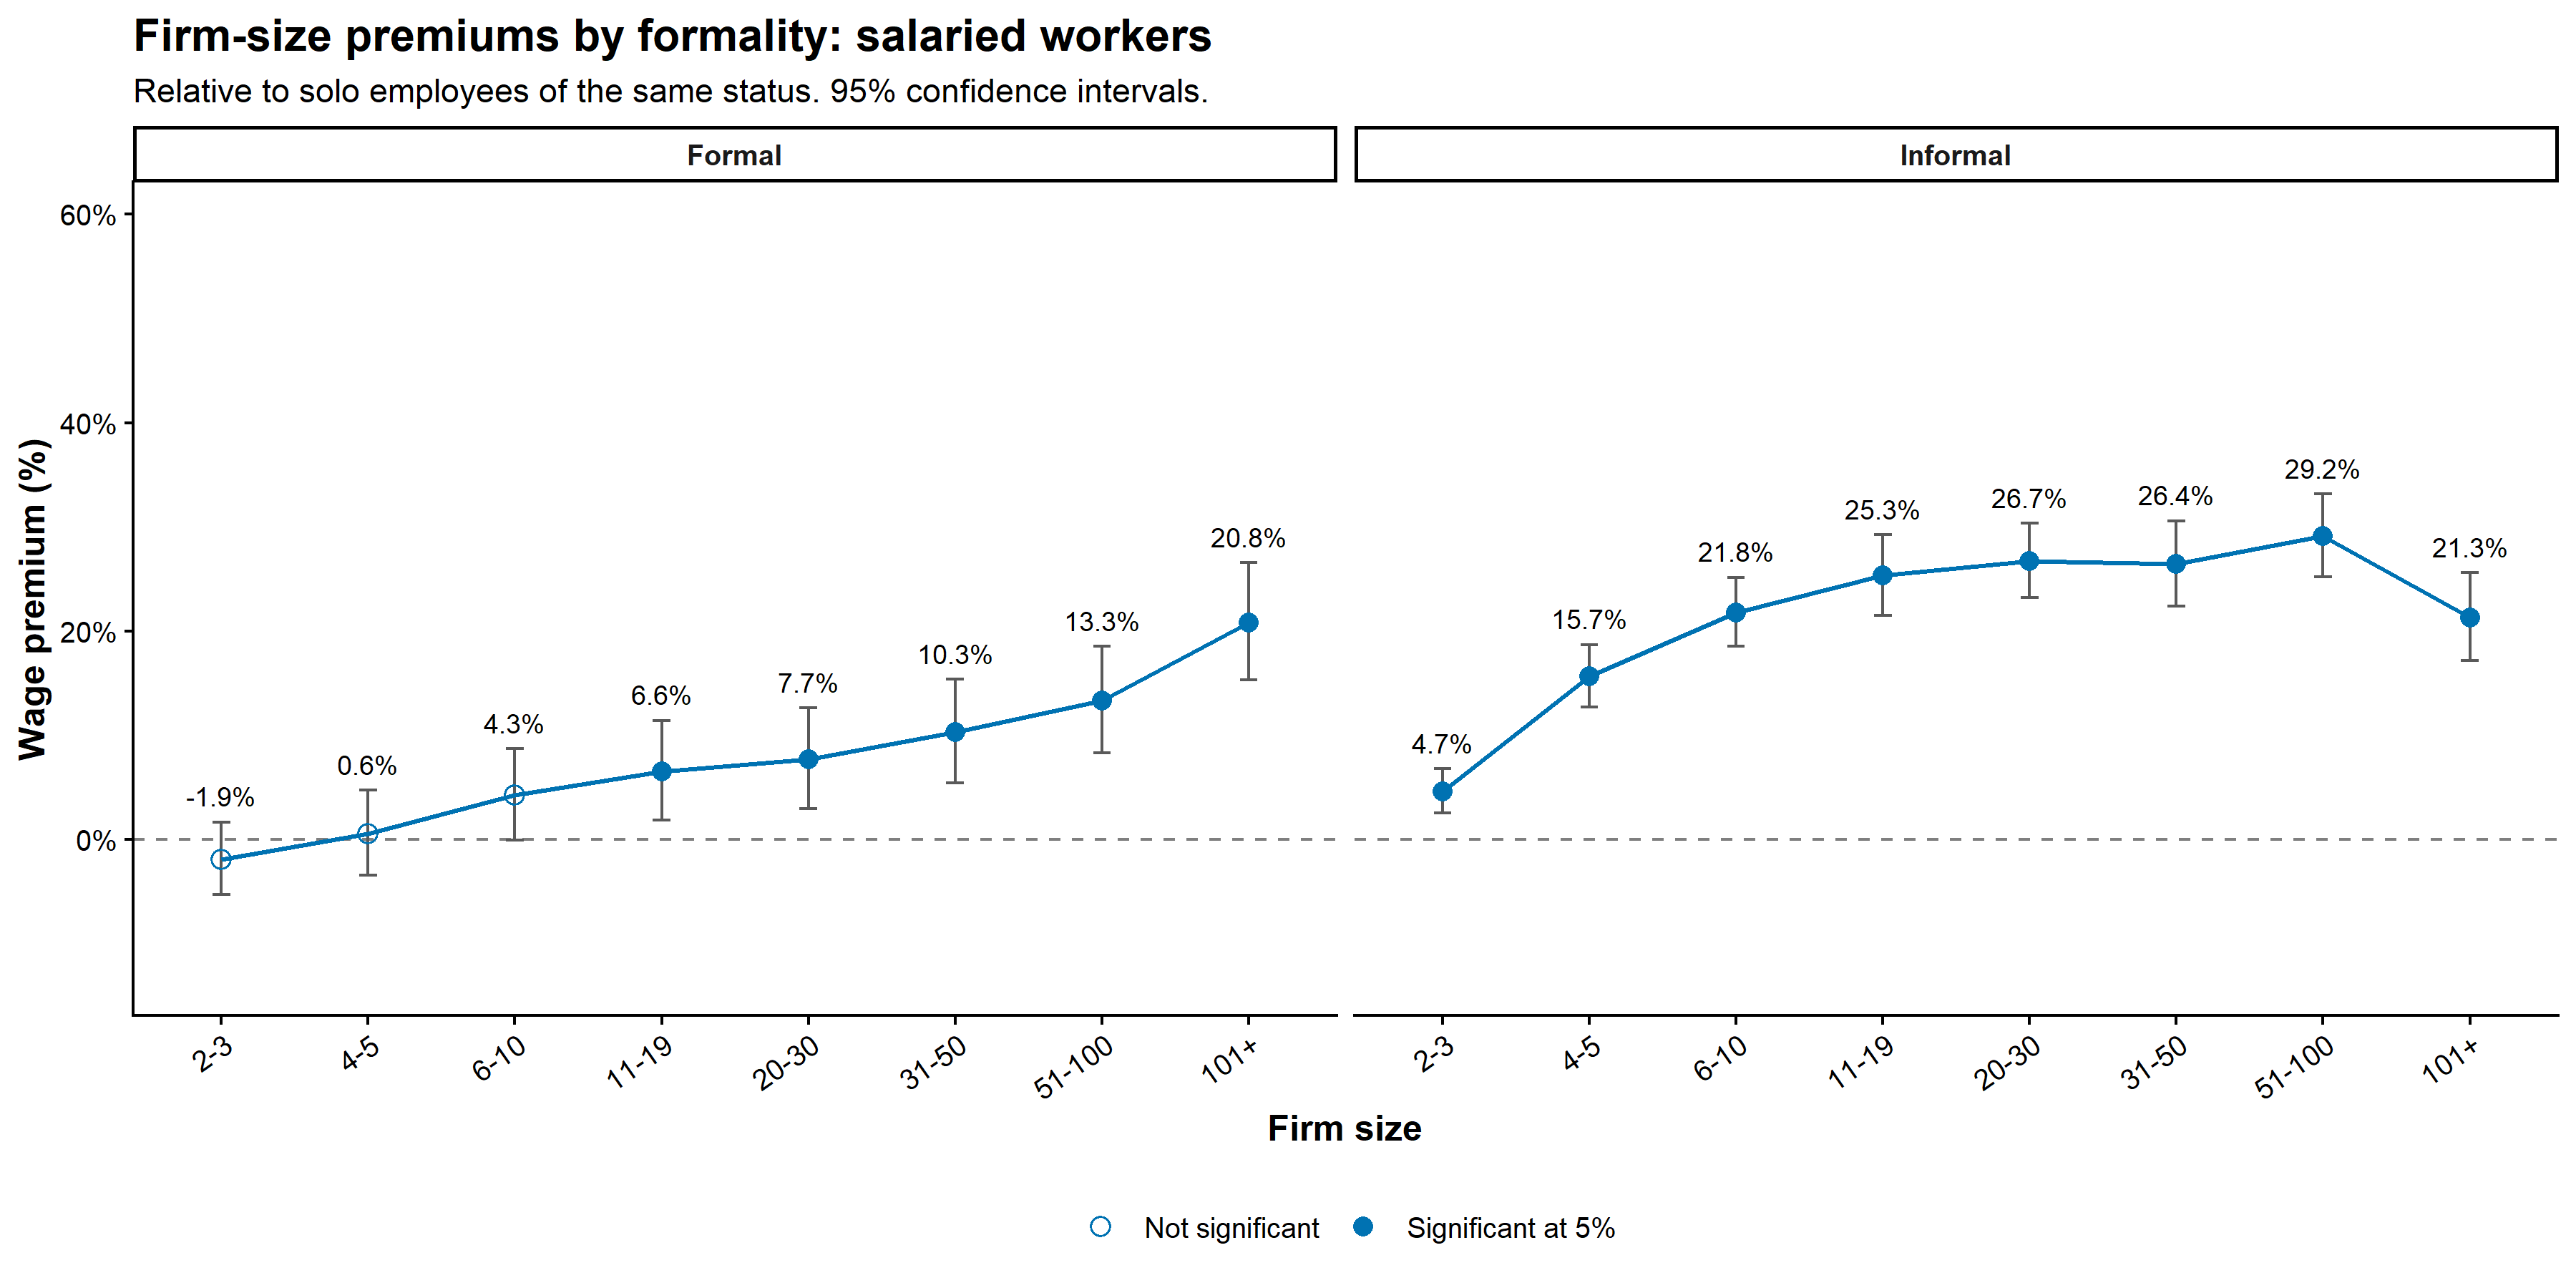
\includegraphics[width=0.98\textwidth,height=0.80\textheight,keepaspectratio]{salaried_formality_premiums_en.png}
  \source{Paper Figure~\paperref{fig:salaried-formality-premium}, Equation~(\paperref{eq:main}) on salaried workers. Same scale as Figure~\paperref{fig:preferred-formality-premium}. Reference is solo work within formality. Intervals use sector-department clustering.}
\end{frame}

\begin{frame}{Salaried-Worker Regression Output}
  \centering\small
  \begin{tabular}{lcc}
  \toprule
  Firm size & Informal & Formal \\
  \midrule
  Solo & -0.226*** \sereg{0.016} & -0.064*** \sereg{0.023} \\
  2--3 & -0.180*** \sereg{0.011} & -0.082*** \sereg{0.013} \\
  4--5 & -0.080*** \sereg{0.007} & -0.058*** \sereg{0.007} \\
  6--10 & -0.028*** \sereg{0.005} & -0.022*** \sereg{0.006} \\
  11--19 & Reference & Reference \\
  20--30 & 0.011* \sereg{0.007} & 0.011*** \sereg{0.003} \\
  31--50 & 0.009 \sereg{0.010} & 0.035*** \sereg{0.004} \\
  51--100 & 0.030** \sereg{0.012} & 0.062*** \sereg{0.006} \\
  101+ & -0.033** \sereg{0.017} & 0.125*** \sereg{0.012} \\
  \bottomrule
  \end{tabular}
  \par\vspace{0.15cm}
  \regnote{Log contrasts relative to 11--19 employees of the same formality status. Standard errors use 555 sector-department clusters. * $p<0.10$, ** $p<0.05$, *** $p<0.01$.}
\end{frame}

\begin{frame}{Similar Endpoints Do Not Mean Identical Profiles}
  \centering\small
  \begin{tabular}{lrrrr}
  \toprule
   & \multicolumn{2}{c}{All workers} & \multicolumn{2}{c}{Salaried workers} \\
   & Formal & Informal & Formal & Informal \\
  \midrule
  101+/solo premium & 17.2\% & 37.0\% & 20.8\% & 21.3\% \\
  11--19/solo premium & 4.2\% & 42.5\% & 6.6\% & 25.3\% \\
  \bottomrule
  \end{tabular}
  \par\vspace{0.3cm}
  \begin{itemize}
    \item Among employees, equality of the formal and informal 101+/solo contrasts is not rejected ($p=0.888$).
    \item Equality of all eight size contrasts is rejected jointly ($p<0.001$).
    \item Both conclusions hold with sector clustering too.
  \end{itemize}
  \source{Paper Table~\paperref{tab:salaried-robustness}. The restricted-sample comparison does not identify a causal contribution of self-employment.}
\end{frame}

\begin{frame}{Changes over Time in the Two Samples}
  \centering\small
  \begin{adjustbox}{max width=\textwidth}
    \begin{tabular}{@{}llrrrrr@{}}
\toprule
    & & \multicolumn{2}{c}{Premium (\%)} & & \multicolumn{2}{c}{$p$-value of change} \\
    \cmidrule(lr){3-4}\cmidrule(lr){6-7}
    Sample & Status & 2008 & 2025 & \shortstack{Change\\(pp)} & \shortstack{Sector-\\department} & Sector \\
    \midrule
All workers & Formal & 16.6 & 13.5 & -3.2 & 0.467 & 0.527 \\
& Informal & 33.2 & 57.1 & 23.8 & 0.002 & 0.040 \\
\midrule
    Salaried workers & Formal & 15.4 & 19.0 & 3.5 & 0.498 & 0.458 \\
& Informal & 22.9 & 39.0 & 16.1 & 0.061 & 0.156\\
\bottomrule\end{tabular}

  \end{adjustbox}
  \par\vspace{0.3cm}
  \begin{itemize}
    \item The informal estimate increases in both samples. Among salaried workers, the change is not significant at 5\% with sector-department or sector clustering.
    \item Formal changes are not significant in either sample. These endpoint comparisons do not establish a steady trend.
  \end{itemize}
  \source{Paper Table~\paperref{tab:salaried-dynamic-comparison}. Tests concern changes in log-wage contrasts.}
\end{frame}

\begin{frame}{Income Scenarios for Salaried Workers}
  \centering\small
  \setlength{\tabcolsep}{4pt}
  {\small Salaried workers represented in 2025: 12.71 million.\par}
\vspace{0.2cm}
\begin{tabular}{p{0.36\textwidth}rrr}
\toprule
Allocation & \shortstack{Workers\\reassigned\\(millions)} & \shortstack{Reassigned workers\\Mean income\\gain (\%)} & \shortstack{All salaried workers\\Total income\\gain (\%)} \\
\midrule
Informal to formal, same size & 4.11 & 23.9 & 4.3 \\
Formal to formal 101+ & 3.57 & 12.8 & 3.6 \\
Informal to informal 101+ & 4.04 & 8.7 & 1.5 \\
\midrule
All workers to formal 101+ & 7.68 & 26.5 & 12.3 \\
\bottomrule\end{tabular}

  \par\vspace{0.3cm}
  {\small Re-estimate the preferred model on salaried workers. The joint total-income change is 12.3\%, compared with 25.9\% in the full sample.\par}
  \source{Paper Table~\paperref{tab:salaried-income-comparison}. Weekly income. Hold hours and estimated coefficients fixed within each sample.}
\end{frame}

\begin{frame}{Why the Aggregate Gains Differ across Samples}
  \begin{itemize}
    \item The full sample includes many low-income non-salaried workers. They account for much of the reassignment in the joint scenario.
    \item Keeping the full-sample coefficients but calculating income changes only for salaried workers gives 13.0\%, close to the 12.3\% from re-estimation.
    \item Much of the difference therefore reflects who enters the income calculation. The sample comparison does not identify a causal effect of self-employment.
  \end{itemize}
  \source{Paper discussion and replication/salaried_extensions_output/income_scenarios.csv, full-sample coefficients applied to salaried workers.}
\end{frame}

\sectionframe{Appendix. Comparison Specifications and Shape Checks}

\begin{frame}{Survey Design and Inference}
  \begin{itemize}
    \item GEIH uses stratified, multistage geographic sampling. The model file lacks the sampling-stratum and primary-unit identifiers.
    \item Clustering checks assess residual dependence, not the exact survey-design variance.
    \item Compare sector-department intersections, sectors, departments, and two-way sector and department clustering.
  \end{itemize}
  \source{Paper Table~\paperref{tab:preferred-clustering-comparison}. Cameron and Miller (2015).}
\end{frame}

% Temporarily omitted from the presentation.
% % Retained for later use, but not included in presentacion_javeriana.tex.
\begin{frame}{Which Comparisons Survive the Bootstrap Checks?}
  \small\centering
  \begin{tabular}{lrrr}
\toprule
Contrast & Premium (\%) & $p$ (sector) & $p$ (two-way) \\
\midrule
Formal 101+/solo & 16.5 & 0.184 & 0.188 \\
Informal 101+/solo & 37.1 & $<0.001$ & $<0.001$ \\
Formal 101+/11--19 & 12.0 & 0.004 & 0.003 \\
Informal 101+/11--19 & -3.7 & 0.217 & 0.210 \\
\bottomrule\end{tabular}

  \par\vspace{0.35cm}
  \begin{itemize}
    \item Coefficients and samples stay fixed. Only inference changes.
    \item There are 559 sector-department intersections, but 17 sectors and 33 departments.
    \item The formal 101+/solo contrast is sensitive. The advantage over intermediate formal categories is not.
  \end{itemize}
  \source{Paper Tables~\paperref{tab:preferred-clustering-comparison}--\paperref{tab:preferred-wild-bootstrap}. Two-sided wild cluster bootstrap, 9,999 draws. Two-way inference allows dependence within sectors and within departments.}
\end{frame}


\begin{frame}{A Common Size Premium across Formality Groups}
  \centering
  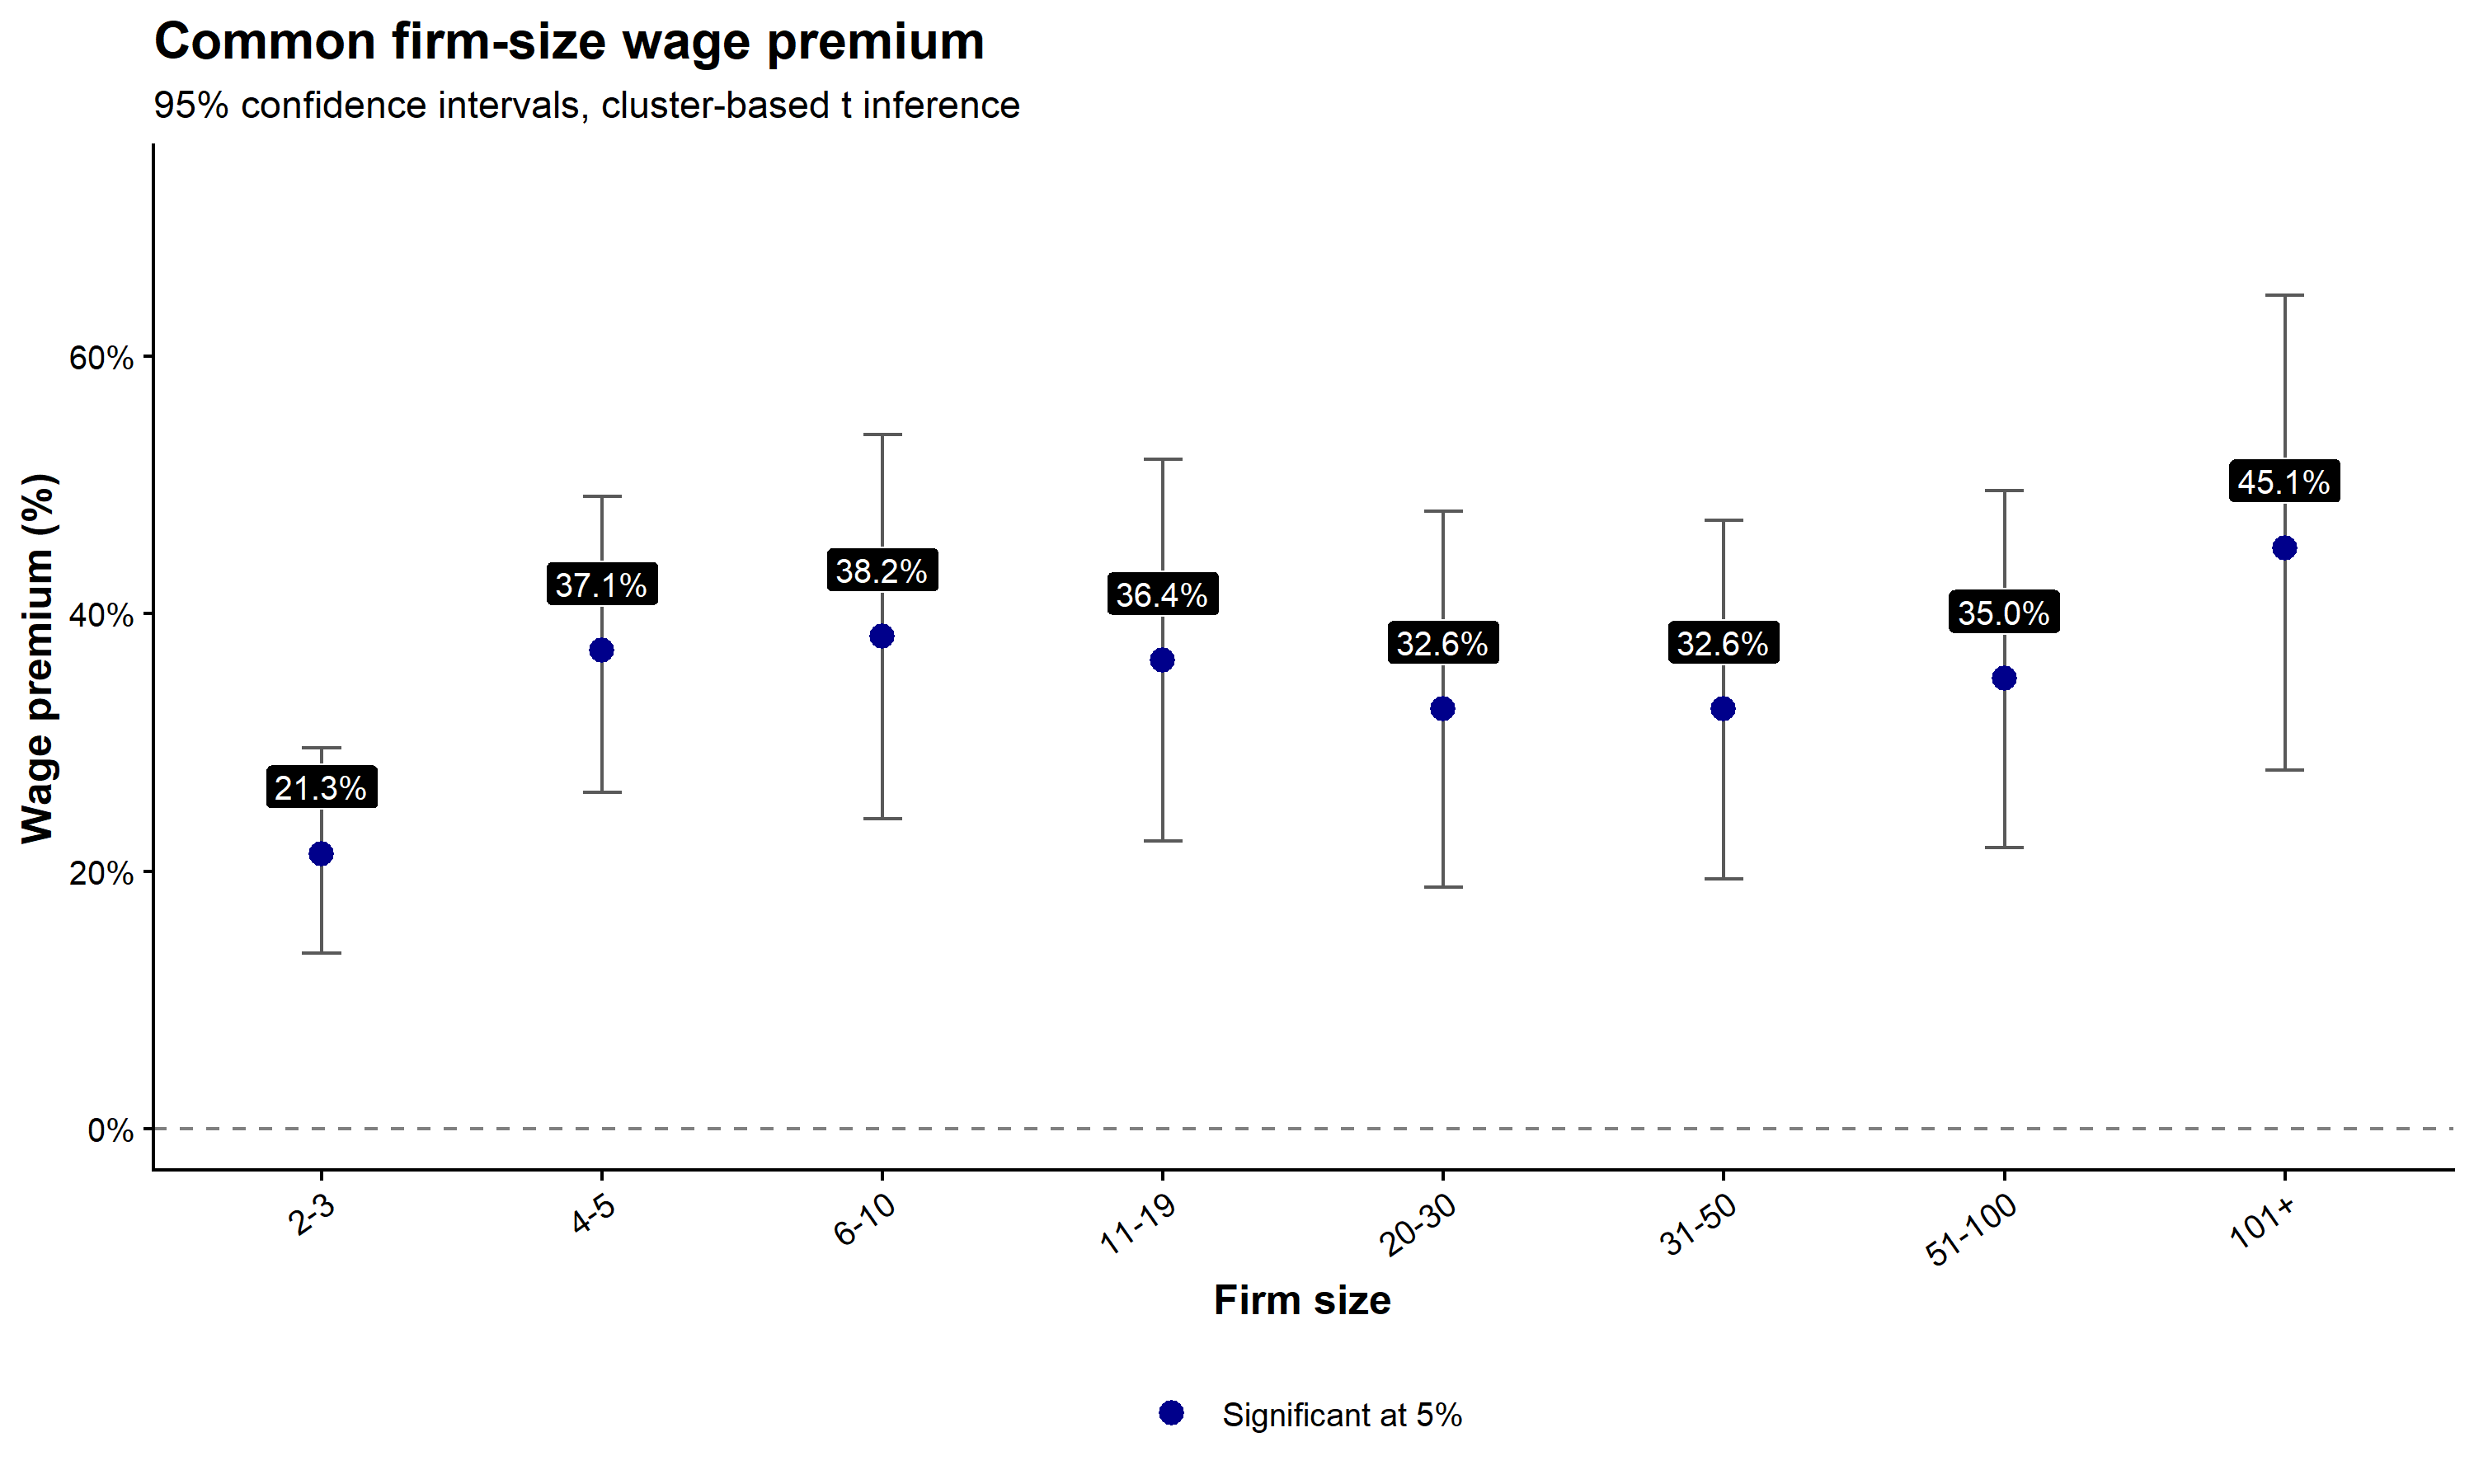
\includegraphics[width=0.98\textwidth,height=0.80\textheight,keepaspectratio]{fig57_en.png}
  \source{Paper Figure~\paperref{fig:firm-size-wage-premium}. Comparison specification with sector-year effects. The fully controlled 101+/solo premium is 45.1\%. This is not the preferred interacted model.}
\end{frame}

\begin{frame}{Size-by-Formality Profiles with Simpler Controls}
  \centering
  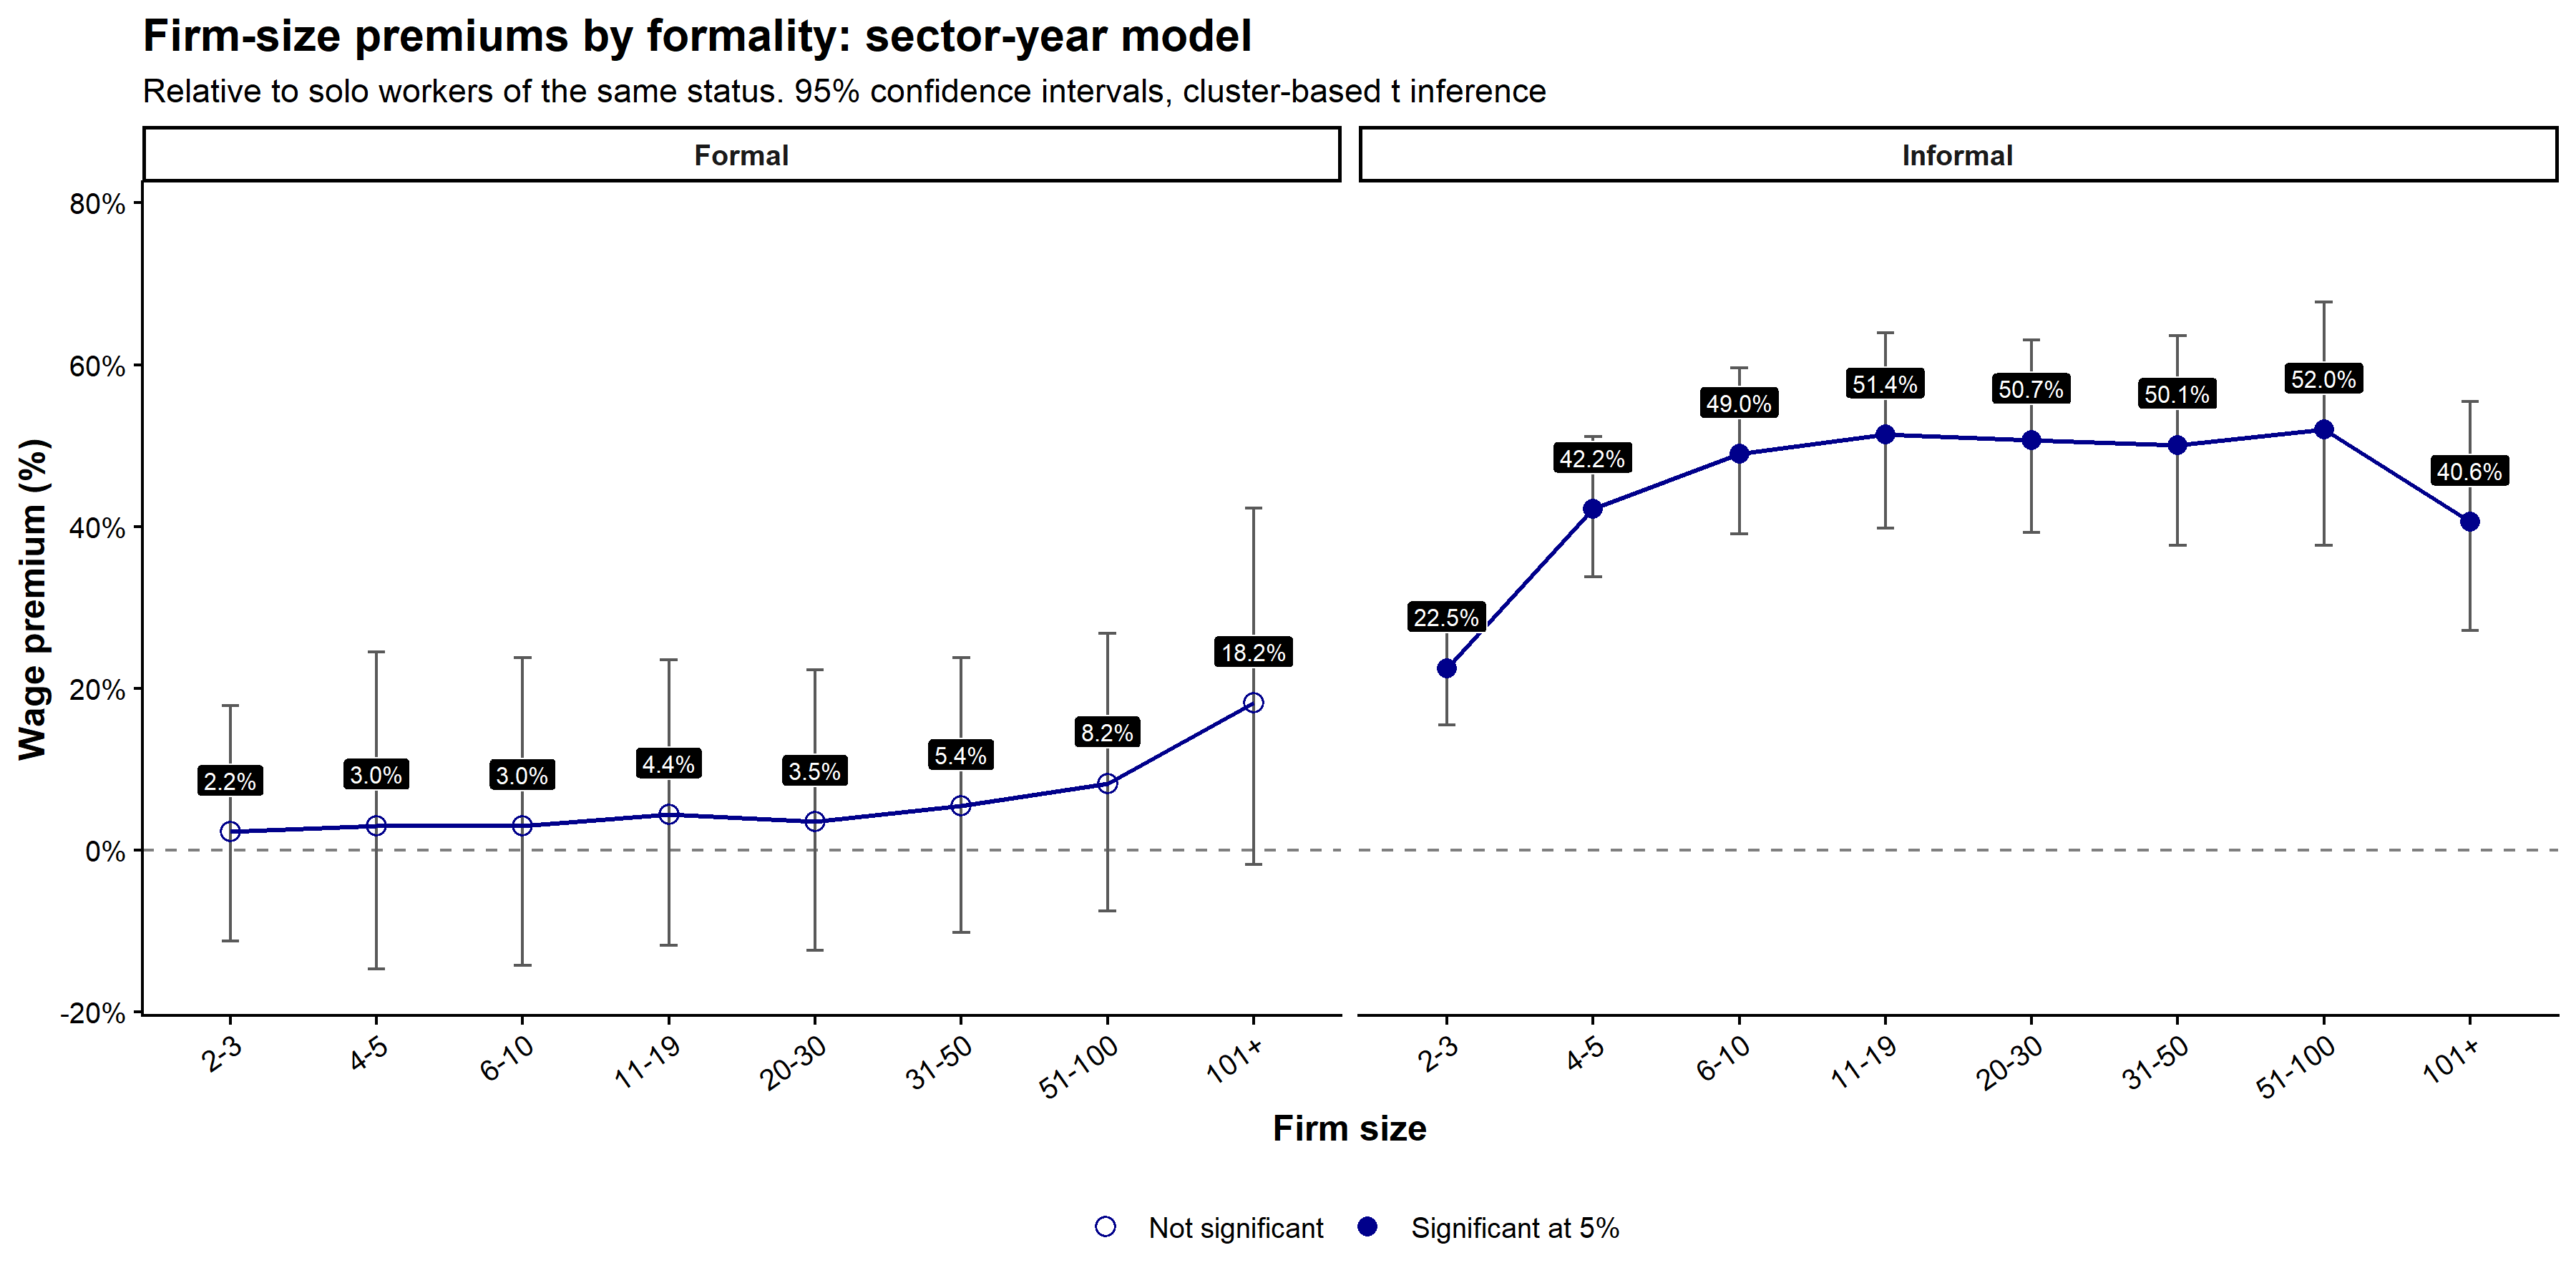
\includegraphics[width=0.98\textwidth,height=0.80\textheight,keepaspectratio]{fig74_en.png}
  \source{Paper Figure~\paperref{fig:firm-size-formality-premium}. Comparison model with worker controls and sector-year effects, without status-in-employment or department controls.}
\end{frame}

\begin{frame}{Dynamics under the Common-Premium Restriction}
  \centering
  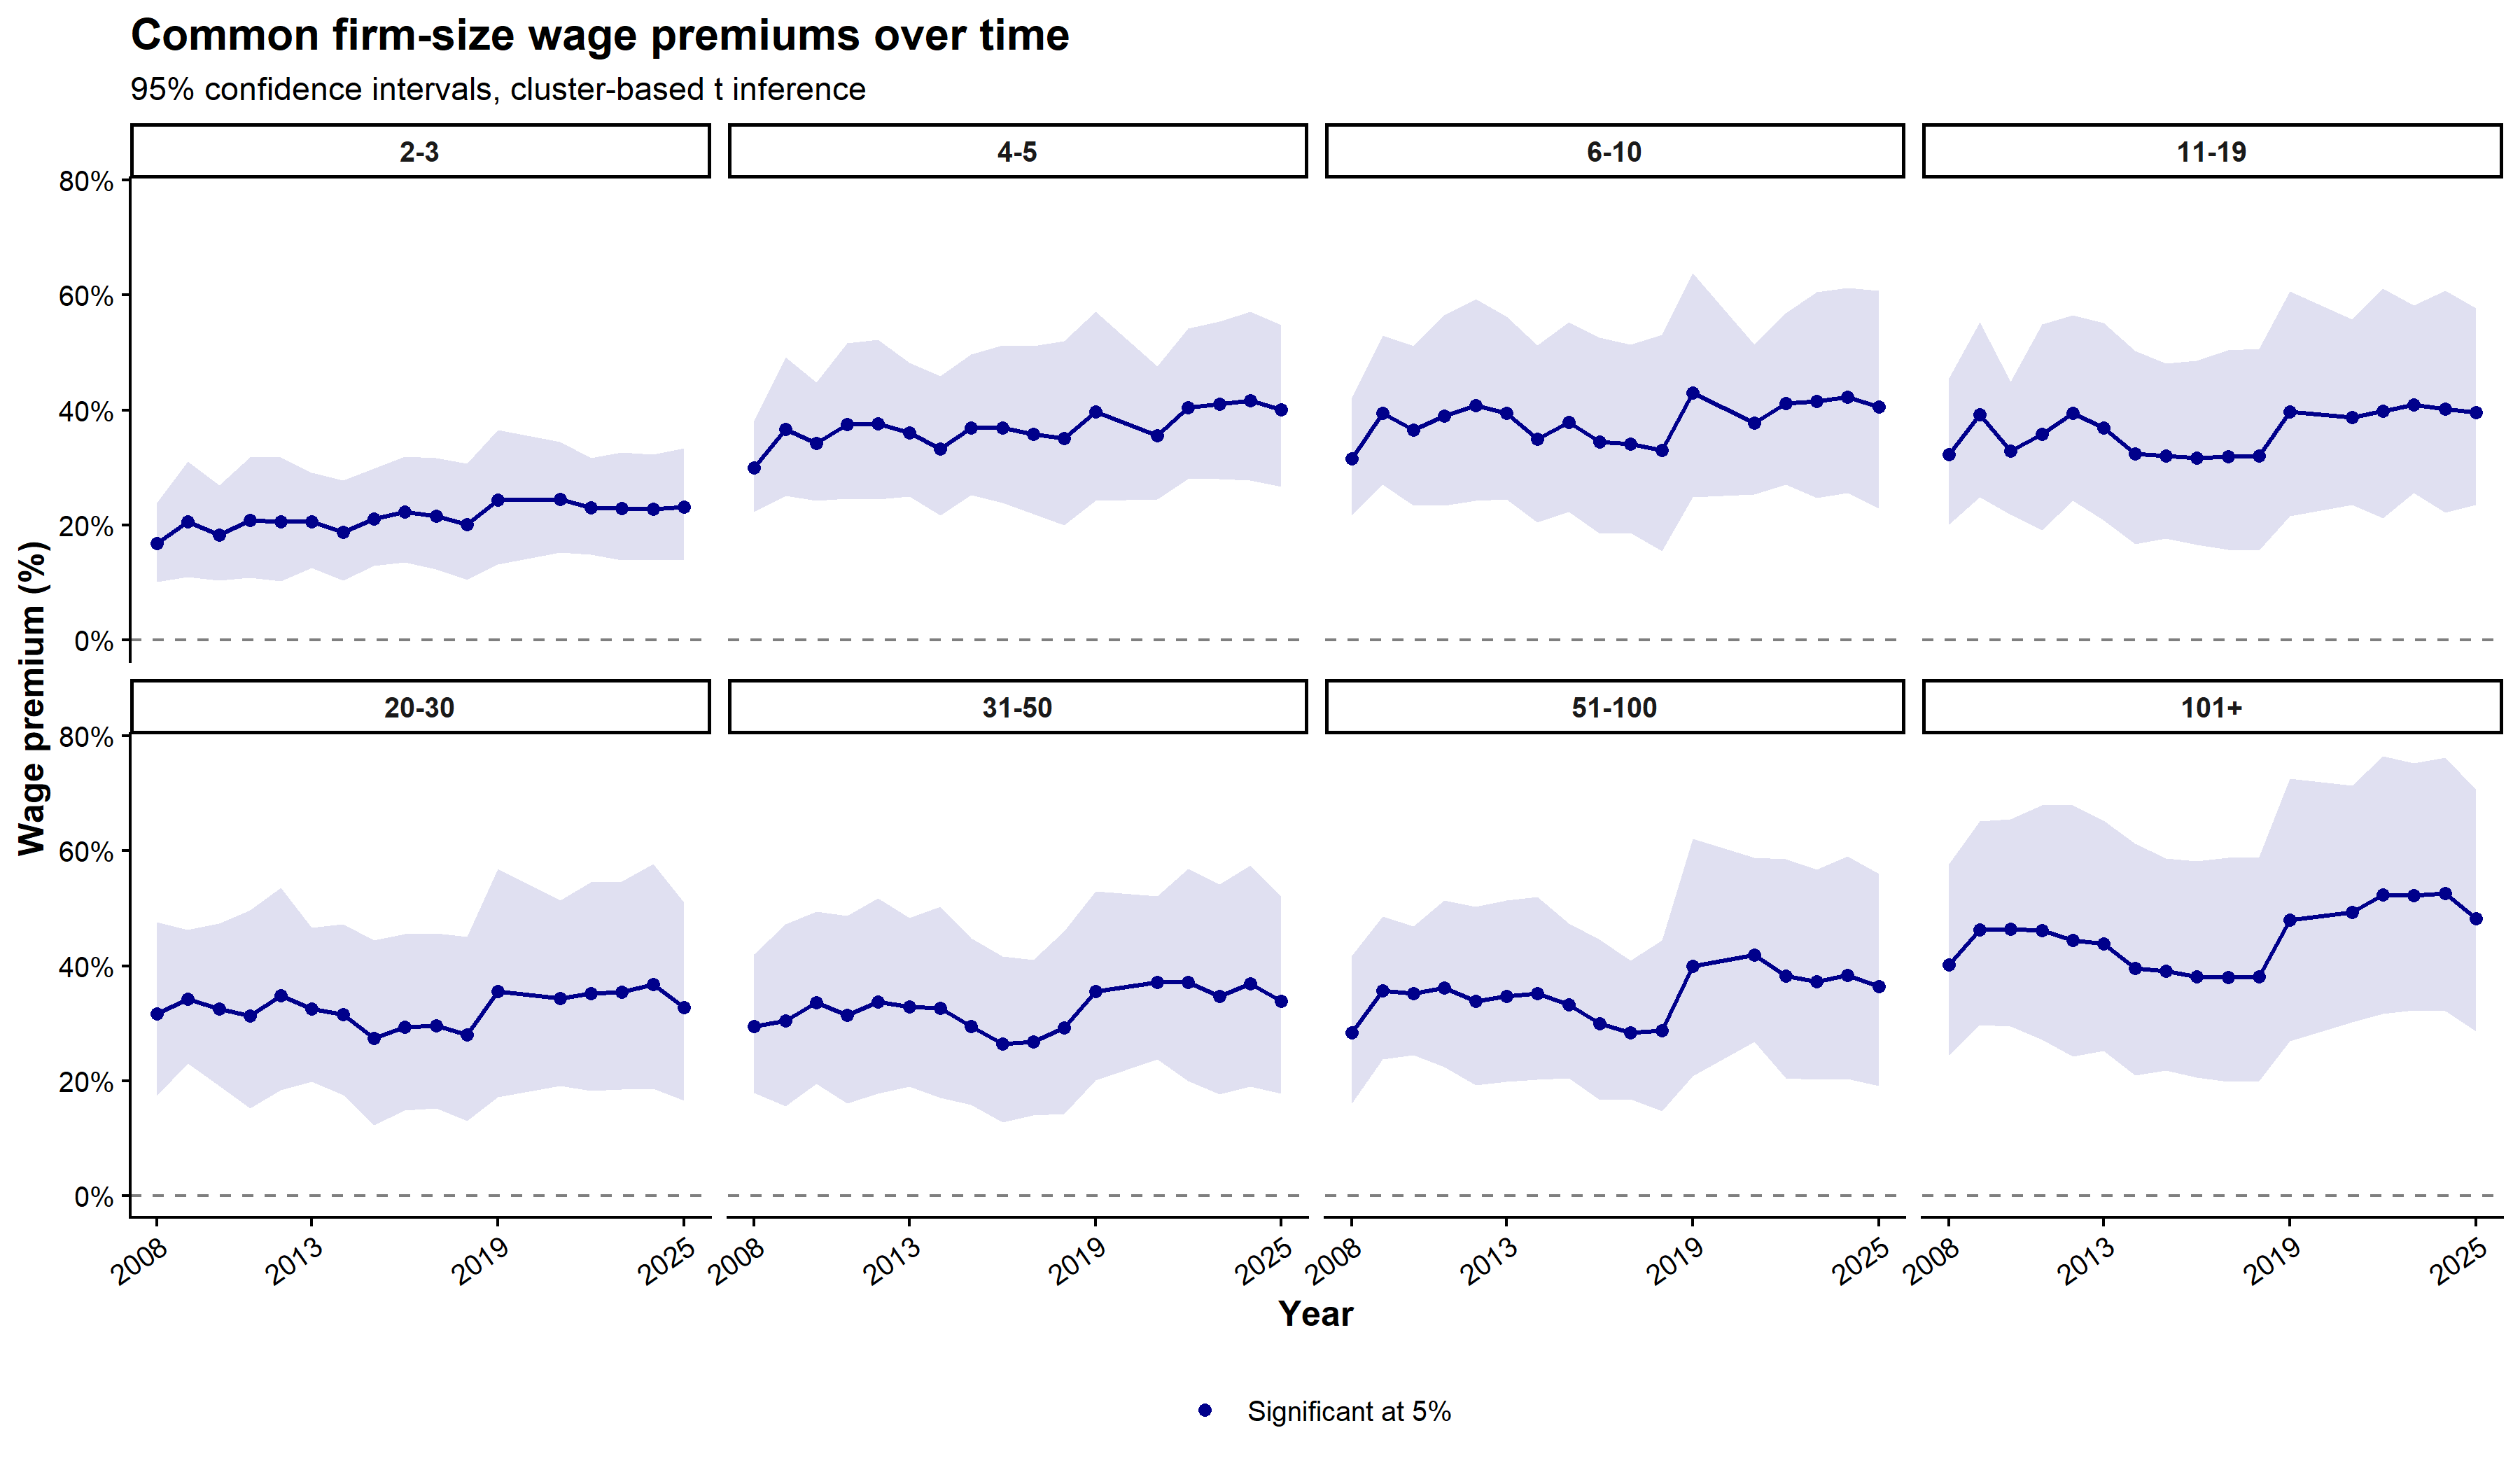
\includegraphics[width=0.98\textwidth,height=0.76\textheight,keepaspectratio]{fig59_en.png}
  \source{Paper Figure~\paperref{fig:firm-size-wage-premium-over-time}. Comparison model with a common size premium across formality groups. Positive but insignificant linear trends do not replace the preferred endpoint tests.}
\end{frame}

\begin{frame}{Formality Endpoints with Simpler Controls}
  \centering
  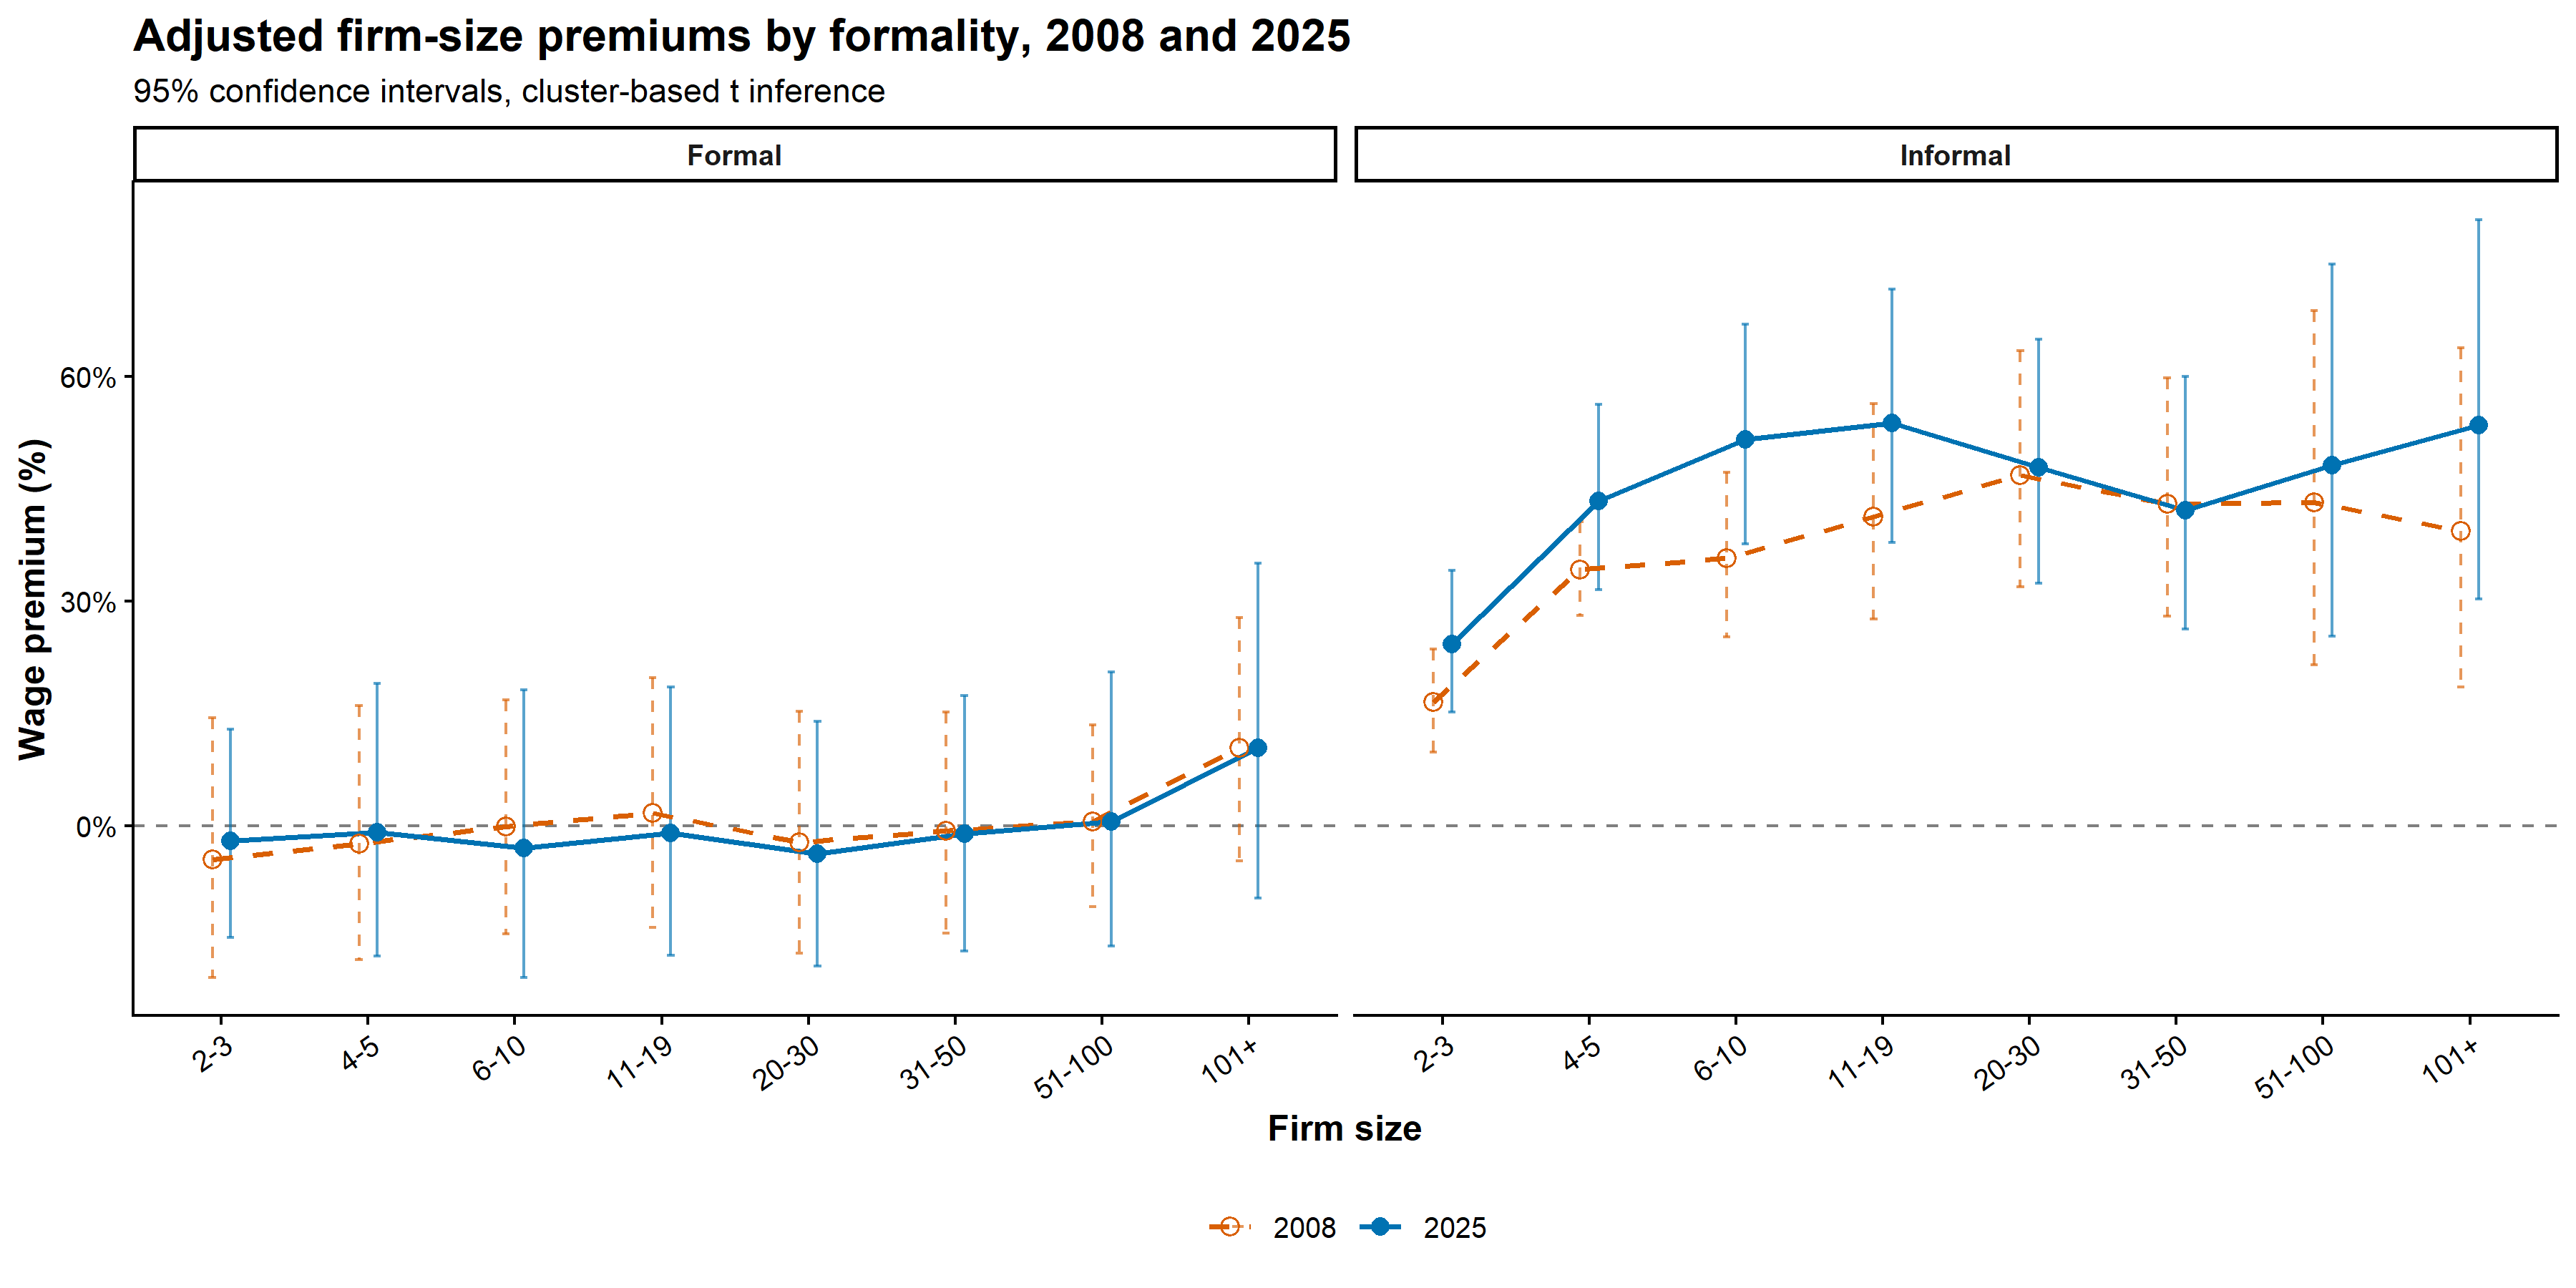
\includegraphics[width=0.98\textwidth,height=0.76\textheight,keepaspectratio]{fig76_en.png}
  \source{Paper Figure~\paperref{fig:adjusted-formality-endpoints}. Equation~(\paperref{eq:formality-interaction}) estimated by year with sector effects, without status-in-employment or department controls. Reference is solo work within each formality-year group.}
\end{frame}

\begin{frame}{Large-Firm Dynamics with Simpler Controls}
  \centering
  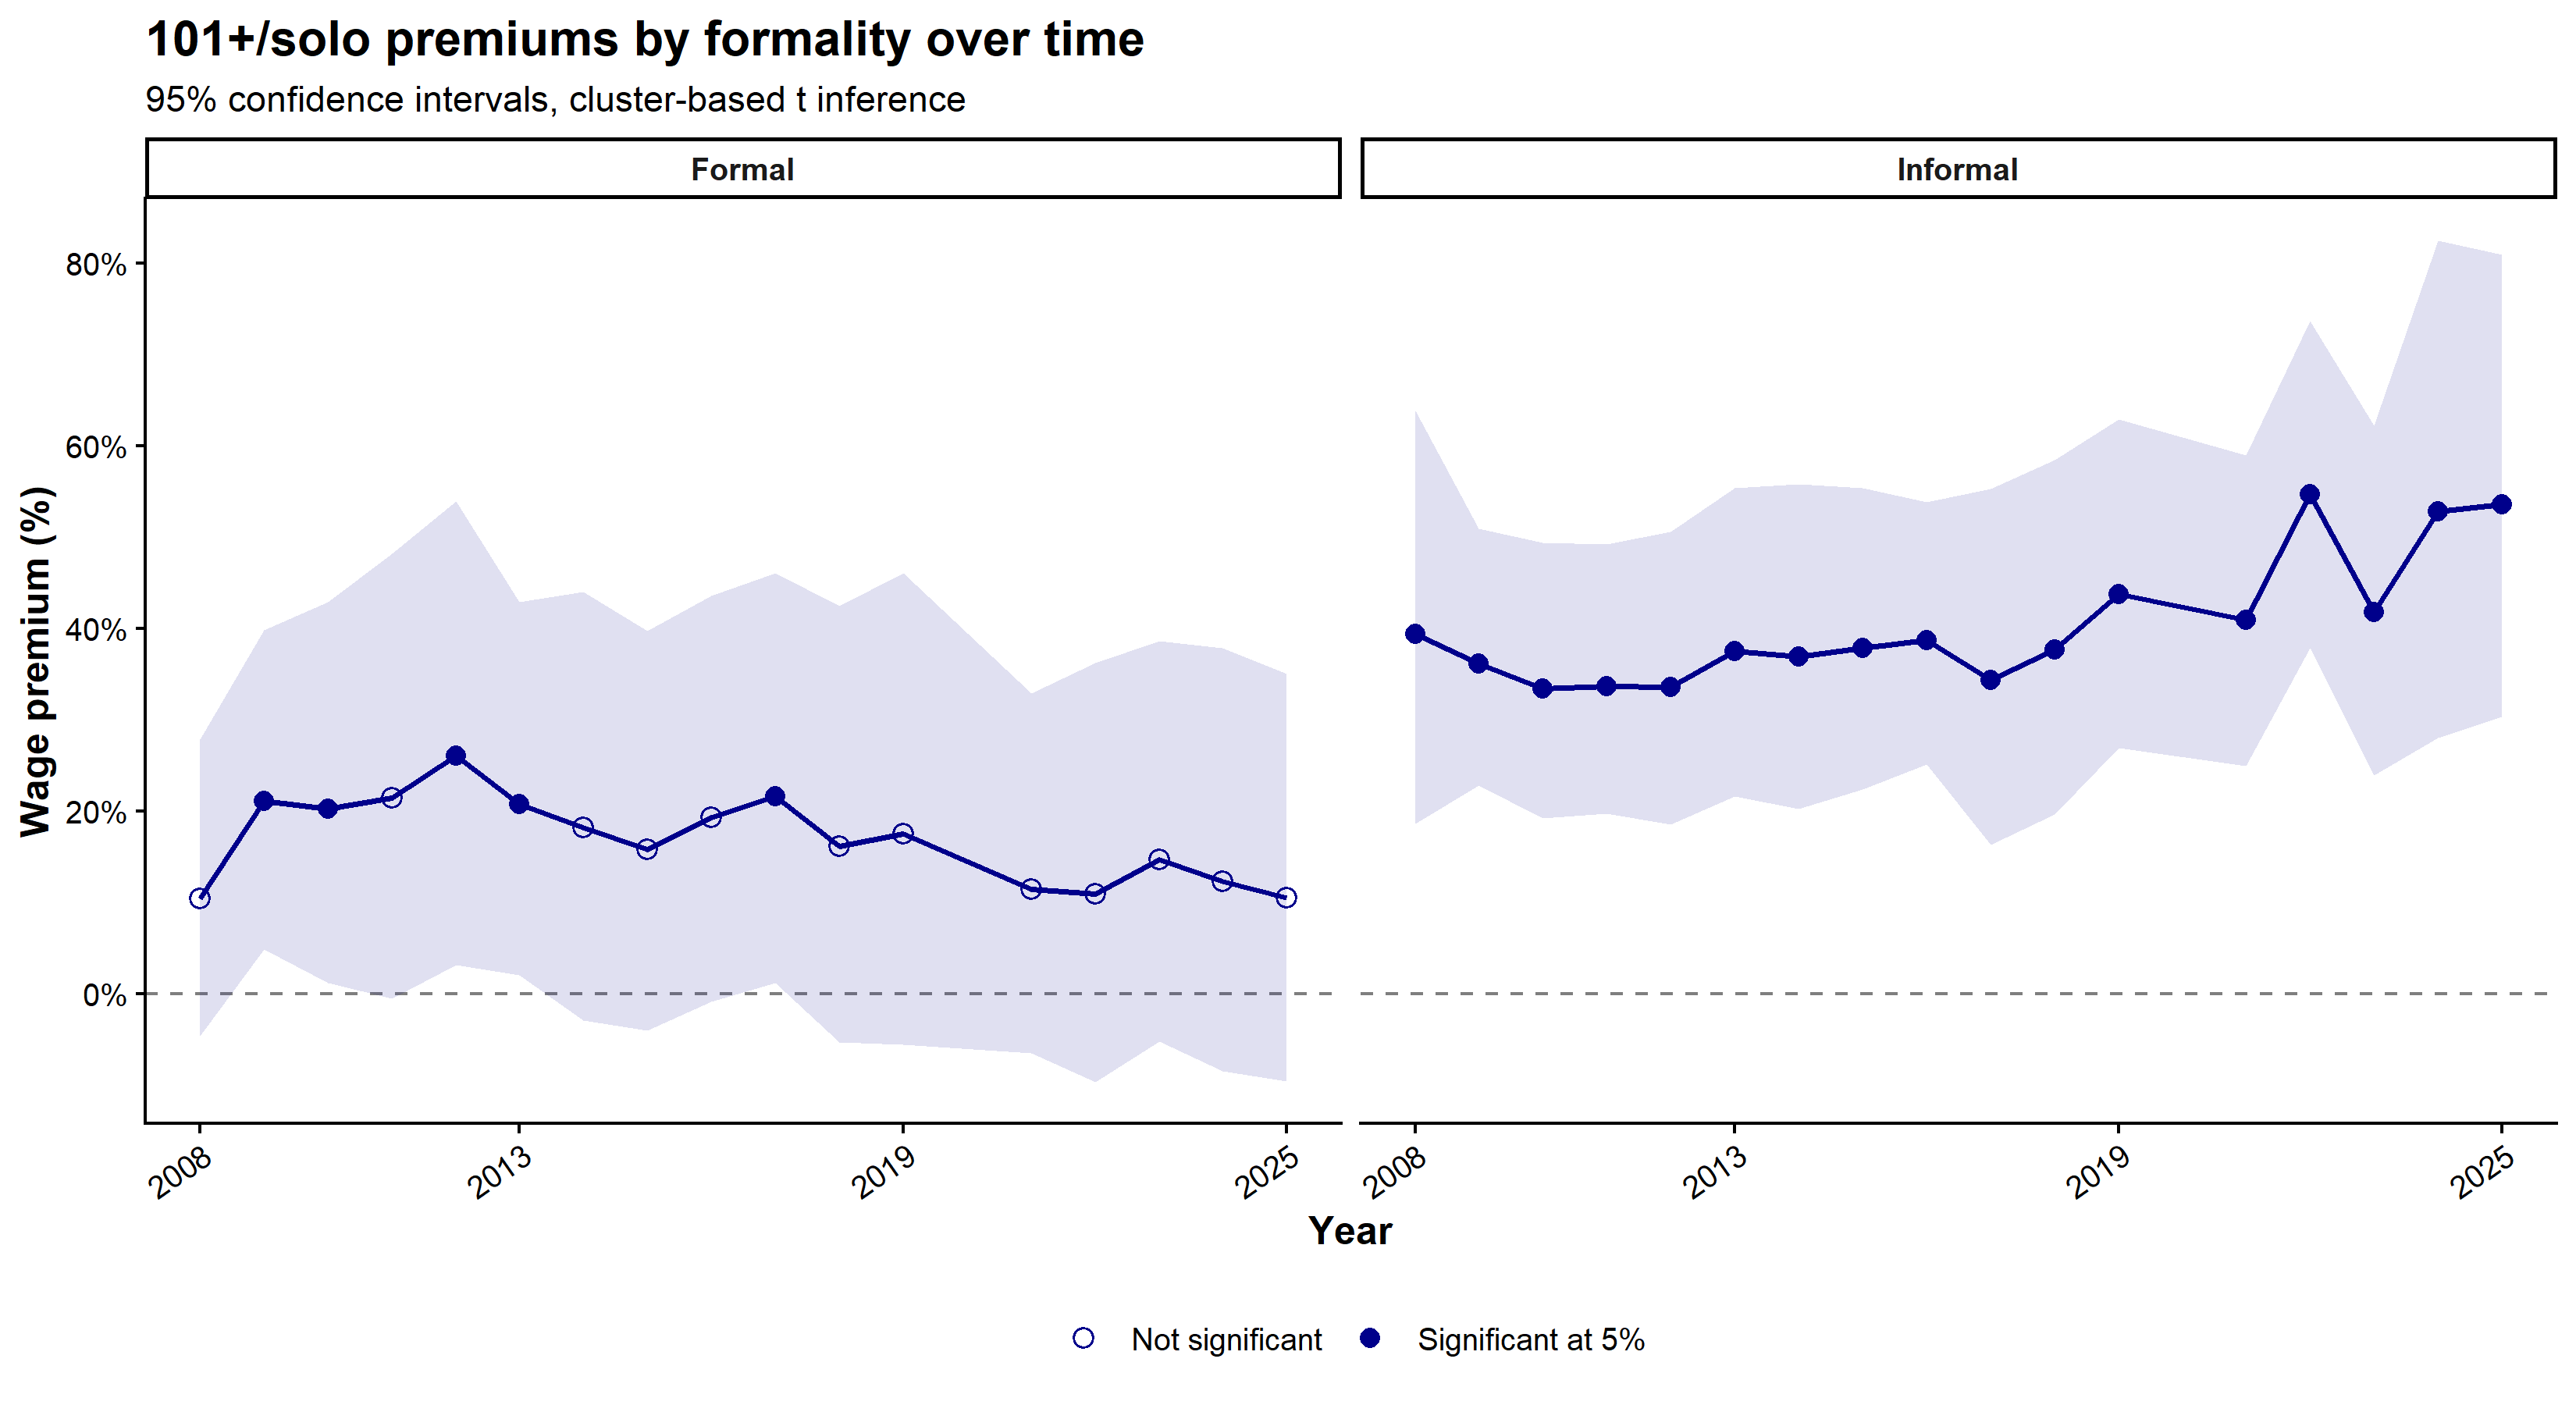
\includegraphics[width=0.98\textwidth,height=0.80\textheight,keepaspectratio]{fig75_en.png}
  \source{Paper Figure~\paperref{fig:large-firm-formality-premium-over-time}. Equation~(\paperref{eq:formality-interaction}) estimated by year with sector effects. Each series compares 101+ workers with solo workers of the same formality status.}
\end{frame}

\begin{frame}{A Quadratic Approximation with Preferred Controls}
  \centering
  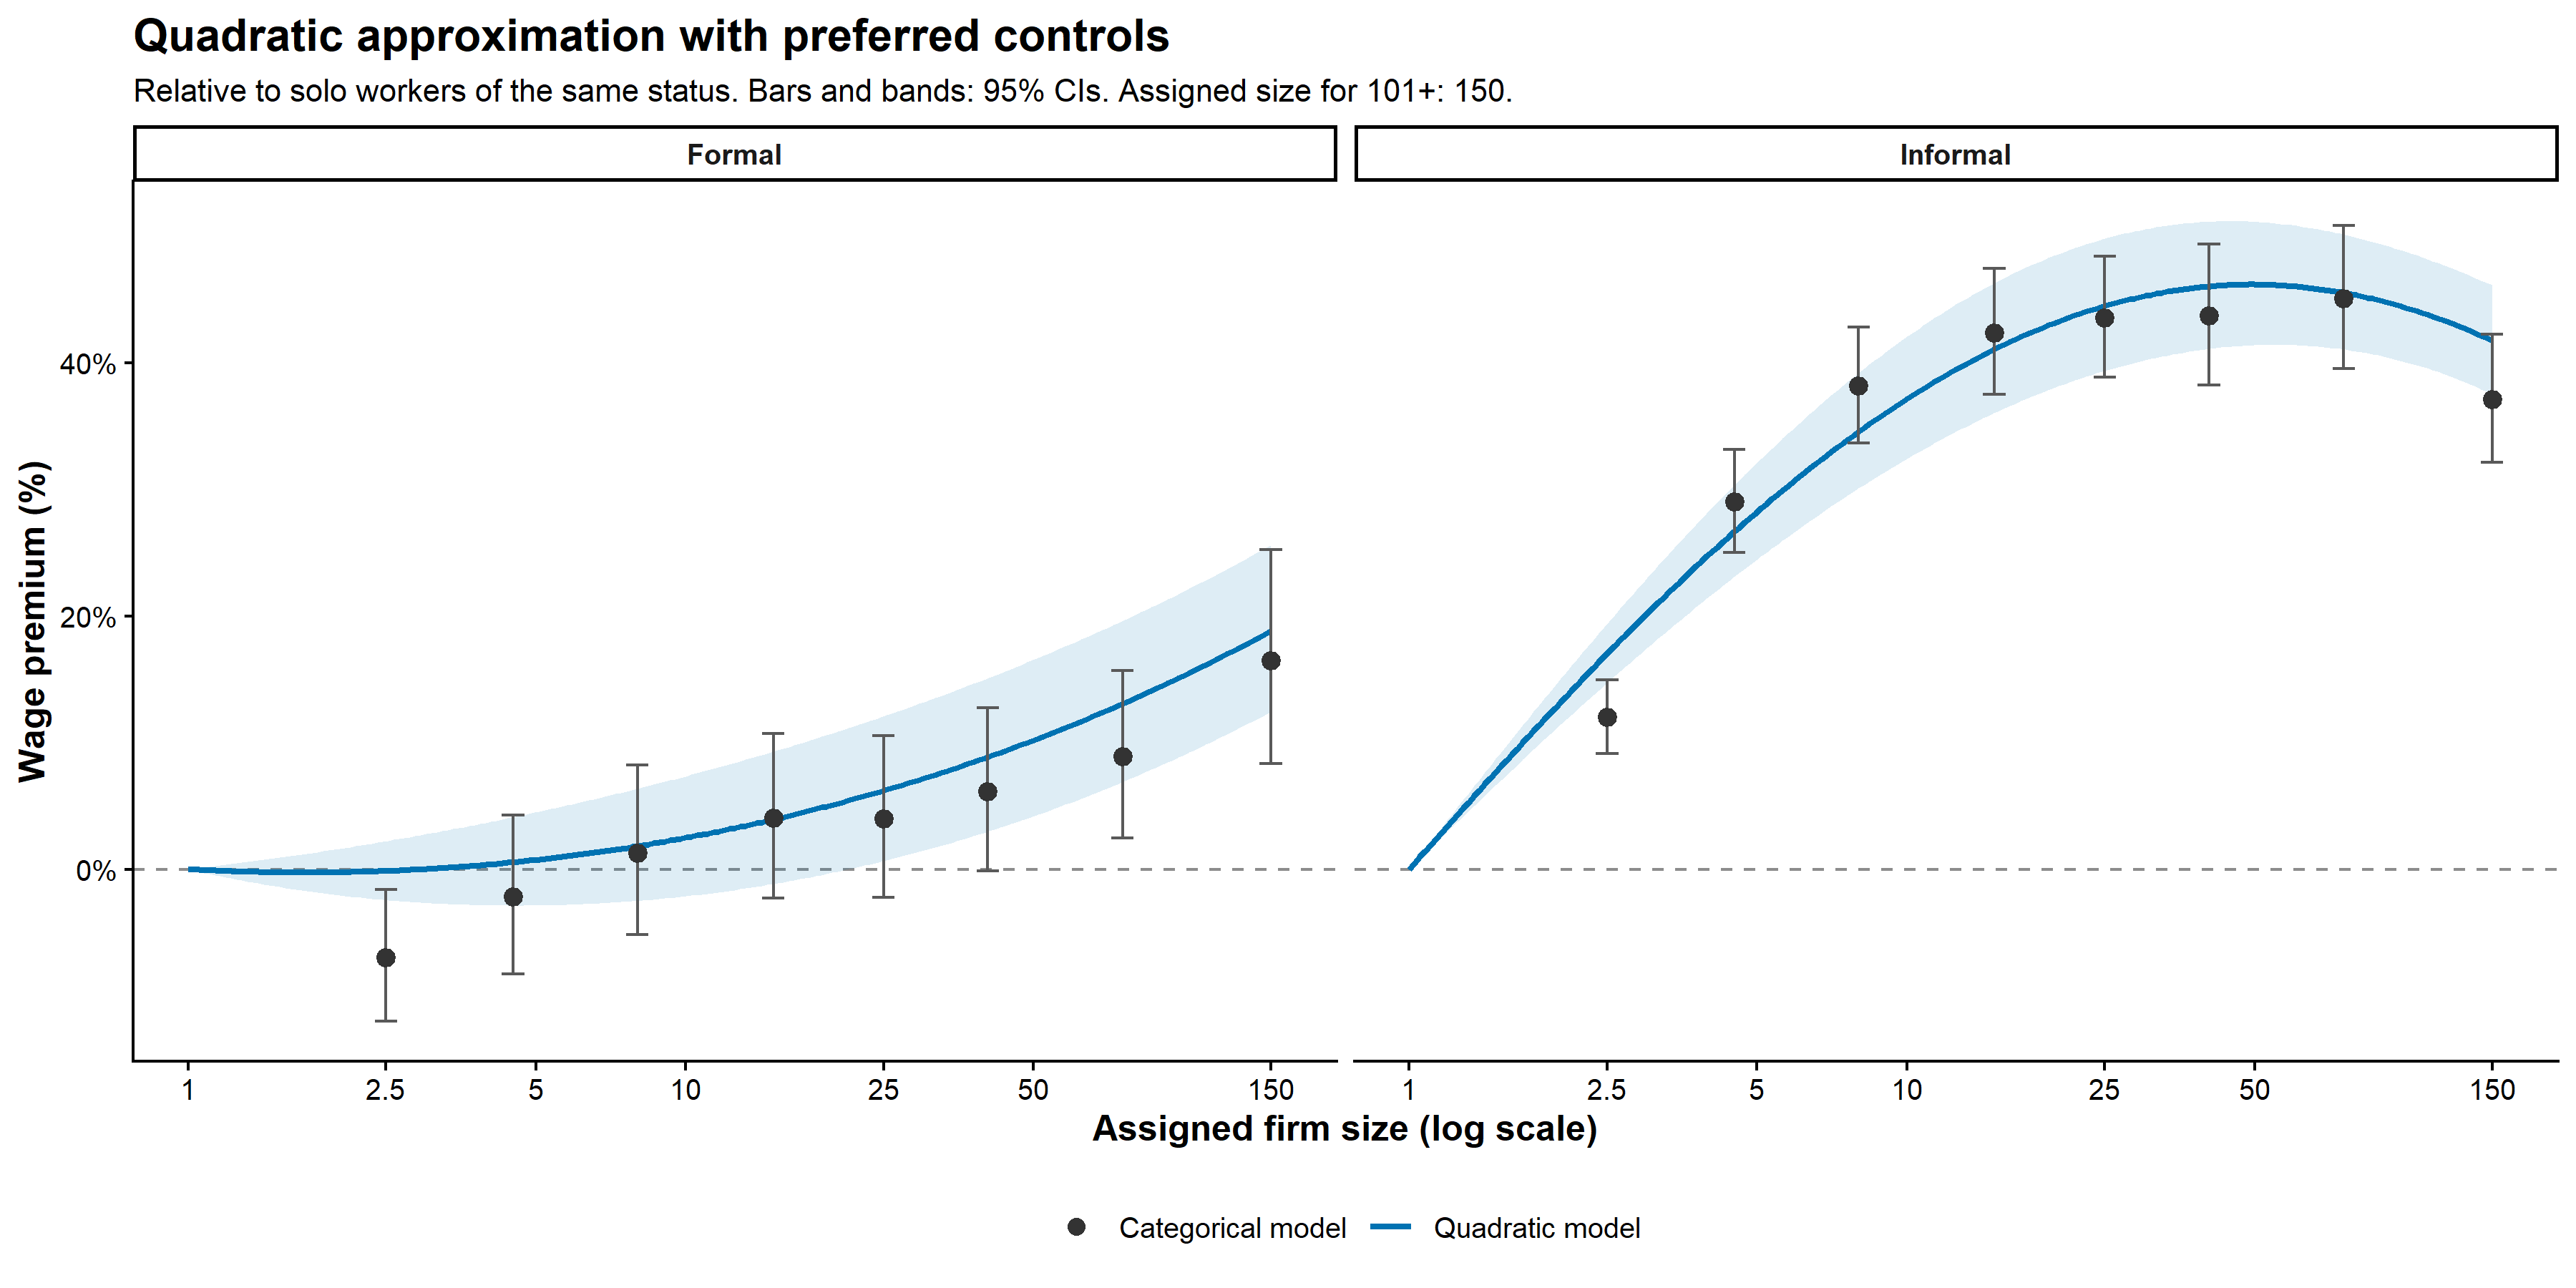
\includegraphics[width=0.98\textwidth,height=0.76\textheight,keepaspectratio]{preferred_quadratic_en.png}
  \source{Paper Figure~\paperref{fig:polynomial-size-profile}. Quadratic in log assigned size, interacted with formality and anchored at solo work. Tables~\paperref{tab:polynomial-size-profile}--\paperref{tab:quadratic-preferred-sensitivity} report coefficients and restriction tests.}
\end{frame}

\begin{frame}{Why Keep the Categorical Model?}
  \begin{itemize}
    \item A low-order polynomial reduces the number of coefficients but imposes a shape on the ordered categories.
    \item We use log assigned size, not the category's ordinal index. The bins have unequal widths.
    \item The quadratic summarizes the broad profiles, but the categorical restrictions are rejected within both formality groups.
    \item The rejection persists when 101+ is assigned 101, 150, or 250 workers. No cubic is fitted.
  \end{itemize}
  \source{Paper Tables~\paperref{tab:polynomial-size-profile}--\paperref{tab:quadratic-preferred-sensitivity}. Fair and Dominguez (1991) motivate the low-order restriction. The categorical specification remains the baseline.}
\end{frame}

\begin{frame}{Why Can Confidence Intervals Overlap?}
  \small
  \[
  \operatorname{Var}(\widehat b_g-\widehat b_h)
  =\operatorname{Var}(\widehat b_g)+\operatorname{Var}(\widehat b_h)
   -2\operatorname{Cov}(\widehat b_g,\widehat b_h).
  \]
  \begin{itemize}
    \item Each plotted interval compares a size category with solo work.
    \item Testing 101+ against 11--19 uses the difference of their coefficients and their covariance.
    \item Overlap between the separate intervals is not a test of that difference.
    \item Changing the reference category gives the same direct contrast and uncertainty.
  \end{itemize}
\end{frame}

\begin{frame}{Selected References}
  \scriptsize
  \begin{itemize}
    \item Balkan, B., and S. Tumen (2016). Firm-Size Wage Gaps along the Formal-Informal Divide: Theory and Evidence. \textit{Industrial Relations}, 55(2), 235--266.
    \item Bloom, N., F. Guvenen, B. S. Smith, J. Song, and T. von Wachter (2018). The Disappearing Large-Firm Wage Premium. \textit{AEA Papers and Proceedings}, 108, 317--322.
    \item Colonnelli, E., J. T{\aa}g, M. Webb, and S. Wolter (2018). A Cross-Country Comparison of Dynamics in the Large Firm Wage Premium. \textit{AEA Papers and Proceedings}, 108, 323--327.
    \item Diegmann, A., S. M\"uller, and B. Schoefer (2026). Off the Labor Supply Curve: The Zero Employer Size Wage Effect Within Large Firms. \textit{NBER Working Paper} 35265.
    \item Fair, R. C., and K. M. Dominguez (1991). Effects of the Changing U.S. Age Distribution on Macroeconomic Equations. \textit{American Economic Review}, 81(5), 1276--1294.
    \item Hsieh, C.-T., and P. J. Klenow (2009). Misallocation and Manufacturing TFP in China and India. \textit{Quarterly Journal of Economics}, 124(4), 1403--1448.
    \item OECD (2026). \textit{OECD Compendium of Productivity Indicators 2026}, Figure 2.1. OECD Publishing. \href{https://doi.org/10.1787/734a5e68-en}{doi:10.1787/734a5e68-en}.
    \item Reed, T., and T. T. Tran (2019). The Large-Firm Wage Premium in Developing Economies. \textit{World Bank Policy Research Working Paper} 8997.
  \end{itemize}
\end{frame}
